\documentclass[10pt]{cekarticle}
\usepackage{color}
\usepackage{amsmath}
\usepackage{amssymb}

\begin{document}

\title{Proposal for a Minimal SBML Level 2 Definition}

\author{Michael Hucka and Herbert Sauro\\[5pt]
\emph{\normalsize with material taken from other proposals by Andrew Finney},\\[-2pt]
\emph{\normalsize Victoria Gor, Eric Mjolsness and Hamid Bolouri}}

\authoremail{\{mhucka,hsauro\}@cds.caltech.edu}

\address{Systems Biology Workbench Development Group\\
  ERATO Kitano Systems Biology Project\\
  Control and Dynamical Systems, MC 107-81\\
  California Institute of Technology, Pasadena, CA 91125, USA\\[3pt]
  {\url{http://www.cds.caltech.edu/erato}}}

\acknowledge{Principal Investigators: John Doyle and Hiroaki Kitano}

\maketitle

%=============================================================================
% Body.
%=============================================================================

\section{Introduction}

The SBML community is currently engaged in defining extensions to SBML
Level~1~\citep{hucka:2001g} to support the representation of many new
features: spatial geometry, model layout/diagrams, metadata, arrays,
multistate biochemical entities, etc.  All the features are important and
will ultimately be necessary; however, for practical reasons, we propose
here an alternative definition of Level~2 containing only a modest subset
of features, with others left to SBML Level~3.  The motivations for this
proposal are the following:
\begin{enumerate}
  
\item A limited target for Level 2, containing a small set of features, can
  act as a concrete milestone on the road to developing a fuller Level~3
  definition.
  
\item A smaller set of new SBML features to consider will enable the
  community to better evaluate the effects of the proposed changes and
  additions.

\item With a smaller set of changes to evaluate, it should be possible for
  the SBML community to reach consensus more quickly and define a working
  SBML Level~2 in short order.
  
\item There is currently an opportunity to contribute to the choice of
  exchange languages used by the DARPA BioSPICE effort.  Discussions in the
  BioSPICE community has lead to the suggestion that SBML could be
  sufficient for their needs if it were extended to support the following:
  allowing user-defined functions, allowing discontinuous functions in
  formulas, and supporting simple metadata.  This opportunity will exist
  only for a limited time; therefore, we propose to define Level~2 quickly,
  which is more likely to happen if the increment from Level~1 is kept
  small.

\end{enumerate}

We propose that SBML Level 2 consist of four features added to SBML
Level~1: (1) a convention for encoding arbitrary symbols in the
\texttt{SName} syntax; (2) the provision for conditional expressions in
formula strings; (3) the addition of user-defined functions for formulas;
and (4) the addition of a basic set of metadata.

This proposal is partly based on a previous proposal by
\citet{finney:2002c}.  In order to provide readers with a self-contained
proposal, we incorporate portions of Finney et al.'s document directly in
this one.


\section{Features Proposed for SBML Level 2}

The following sections detail the proposed additions to SBML Level~1.


\subsection{Encoding Arbitrary Symbols in \texttt{SName}}
\label{sec:encoding}

SBML Level~1 stipulates that symbol names must conform to a particular
limited syntax containing only alphanumeric characters and the underscore
(`\texttt{\_}') character.  This was chosen in an attempt to maximize
compatibility between different software tools which may turn the symbols
of an SBML model directly into symbols in (for example) a scripting
language.

To extend the range of symbols that can be expressed in the very limited
\texttt{SName} syntax, we propose the following encoding rule: for any
character that is not one of `\texttt{\_}', a-z, A-Z, or 0-9, express the
character as the sequence \texttt{\_\_u\textit{XXXX}\_\_} (i.e., two
underscores, followed by the letter `u', followed by four hexadecimal
numbers, following by two more underscores), where \texttt{\textit{XXXX}}
is the hexadecimal Unicode encoding of that
character~\citep{unicode:1996,unicode:2002}.  For example, the name
I$\kappa$B turns into \texttt{I\_\_u03BA\_\_B}, with \texttt{03BA} being
the Unicode sequence for the Greek letter $\kappa$.

If a software program can display a symbol as the appropriate glyph, then
it should translate names containing \texttt{\_\_u\textit{XXXX}\_\_} into the
appropriate glyph on the screen.  If a program cannot display the
character, it should leave it as-is.  In that case, users will still be
able to manipulate the name, though the presentation will be less
attractive.



\subsection{Conditional Expressions in Mathematical Formulas}
\label{sec:conditionals}

\citet{finney:2002c} have already proposed an extension to SBML Level~1
formula strings for expressing discontinuous functions.  We agree with that
proposal, and reproduce the text here for easier reading.  The rest of this
section has been taken mostly verbatim from Section~4 of the document by
\citet{finney:2002c}, with changed items shown in {\color{green}green}.


\subsubsection{New Operators}

Table~\ref{tab:operators} shows a possible extended set of operators that
could be available in SBML Level~2.  New operators are shown in
{\color{red}red} and {\color{green}green}.  As in SBML Level~1, these
operators work as defined in the programming language C, except that the
types are always \texttt{double}.  This means that ``0'' is interpreted as
false and all nonzero numbers are interpreted as true.

The operators \verb|&&| and \verb+||+ short-circuit the evaluation of their
second operand depending on the value of the first operand.
({\color{green} This is an optimization that could be left optional,
  because the functions proposed in Section~\ref{sec:functions} cannot have
  side-effects and therefore short-circuiting cannot change the result
  value of an expression.  However, if the definition of functions is
  changed to support multi-line functions with bodies and possible
  side-effects, it will then become necessary to require short-circuiting
  the evaluation of the operators \verb|&&| and \verb+||+.})

\begin{table}[tbh]
  \vspace*{8pt}
  \begin{center}
    \begin{tabular}{>{\ttfamily}lllcl}
      \toprule
      \textbf{Tokens} & \textbf{Operation} & \textbf{Class} & \textbf{Precedence} & \textbf{Associates} \\
      \midrule
      \emph{name} 	& symbol reference & operand & 10 & n/a \\
      (\emph{expression}) & expression grouping & operand & 10 & n/a\\
      \emph{f}(\emph{...}) & function call & prefix & 10 & left\\
      \color{red} ! 	& \color{red} logical not & \color{red} unary & \color{red} 9 & \color{red} right\\
      \color{green} not & \color{green} logical not & \color{green} unary & \color{green} 9 & \color{green} right\\
      - 		& negation & unary & 9 & right\\
      \verb|^| 		& power & binary & 8 & left \\
      * 		& multiplication & binary & 7 & left\\
      / 		& division & binary & 7 & left\\
      + 		& addition & binary & 6 & left\\
      - 		& subtraction & binary & 6 & left\\
      \color{red} <	& \color{red} less than & \color{red} binary & \color{red} 5 & \color{red} left\\
      \color{red} > 	& \color{red} greater than & \color{red} binary & \color{red} 5 & \color{red} left\\
      \color{red} >= 	& \color{red} greater than or equal & \color{red} binary & \color{red} 5 & \color{red} left\\
      \color{red} <= 	& \color{red} less than or equal & \color{red} binary & \color{red} 5 & \color{red} left\\
      \color{red} == 	& \color{red} equality & \color{red} binary & \color{red} 4 & \color{red} left\\
      \color{red} != 	& \color{red} inequality & \color{red} binary & \color{red} 4 & \color{red} left\\
      \color{red} \&\& 	& \color{red} logical and & \color{red} binary & \color{red} 3 & \color{red} left\\
      \color{green} and & \color{green} logical and & \color{green} binary & \color{green} 3 & \color{green} left\\
      \color{red} || 	& \color{red} logical or & \color{red} binary & \color{red} 2 & \color{red} left \\
      \color{green} or 	& \color{green} logical or & \color{green} binary & \color{green} 2 & \color{green} left \\
      \color{red} ? : 	& \color{red} conditional & \color{red} ternary & \color{red} 1 & \color{red} right \color{black} \\
      \bottomrule
    \end{tabular}
  \end{center}
  \caption{A table of the expression operators available in SBML,
    operators proposed in this document are shown in red.  In the
    \textbf{\textrm{Class}} column, ``operand'' implies the construct is an
    operand, ``prefix'' implies the operation is applied to the following
    arguments, ``unary'' implies there is one argument, and ``binary''
    implies there are two arguments.  The values in the
    \textbf{\textrm{Precedence}} column show how the order of different
    types of operation are determined.  For example, the expression $a * b
    + c$ is evaluated as $(a * b) + c$ because the \texttt{*} operator has
    higher precedence.  The \textbf{\textrm{Associates}} column shows how
    the order of similar precedence operations is determined; for example,
    $a - b + c$ is evaluated as $(a - b) + c$ because the $+$ and $-$
    operators are left-associative.  The precedence and associativity rules
    are taken from the C programming language~\protect\citep{harbison:1995},
    except for the symbol \texttt{\^}, which is used in C for a different
    purpose.}
  \label{tab:operators}
\end{table}

\subsubsection{New Function: \texttt{switch}}

In addition to the new operators described above, we propose
to introduce an additional function called \texttt{switch}.
The syntax of this function would be as follows:
\begin{example}
switch(key, match1, result1, ... matchn, resultn, defaultResult);
\end{example}

This function would compare \texttt{key} to the values
\texttt{match1...matchn} and returns the \texttt{result} value immediately
following the matching \texttt{match}\textit{x} argument.  If none of the
\texttt{match}\textit{x} arguments are equal to \texttt{key}, then
\texttt{switch} would return the value of the \texttt{defaultResult}
argument.

The \texttt{switch} function is merely a convenient way of expressing long
sequences of if-then conditions.  The call
\begin{example}
switch(k, m, r, d)
\end{example}
is equivalent to
\begin{example}
(k == m) ? r : d
\end{example}
The call
\begin{example}
switch(k, m1, r1, m2, r2, d)
\end{example}
is equivalent to
\begin{example}
(k == m1) ? r1 : ((k == m2) ? r2 : d)
\end{example}
and so on.

\subsubsection{Issues}

Given that the function \texttt{switch} and the operators
\texttt{<=}, \texttt{>=} and \texttt{!=} are redundant should
they be incorporated into SBML Level 2?


\newpage
\subsection{User-Defined Functions in Mathematical Formulas}
\label{sec:functions}

\citet{finney:2002c} have already proposed an extension to SBML Level~1 to
allow for user-defined functions.  We agree with that proposal, and
reproduce the text here with one alteration: the addition of two
more questions for dicussion in Section~\ref{sec:function-issues} below.  The
rest of this section has been taken mostly verbatim from Section~5 of the
document by \citet{finney:2002c}.

The proposed redefinition of the \texttt{Model} type is shown in UML in
Figure~\ref{fig:model}.  The change in this new definition is that a
\texttt{Model} can now optionally contain a list of \texttt{Function}
elements.  The definition of \texttt{Function} is shown in
Figure~\ref{fig:function}.

\begin{figure}[h]
  \vspace*{8pt}
  \centering
  
\includegraphics[scale = 0.7]{model}
  \caption{The definition of the \texttt{Model} type.}
  \label{fig:model}
\end{figure}

\begin{figure}[h]
  \vspace*{15pt}
  \centering
  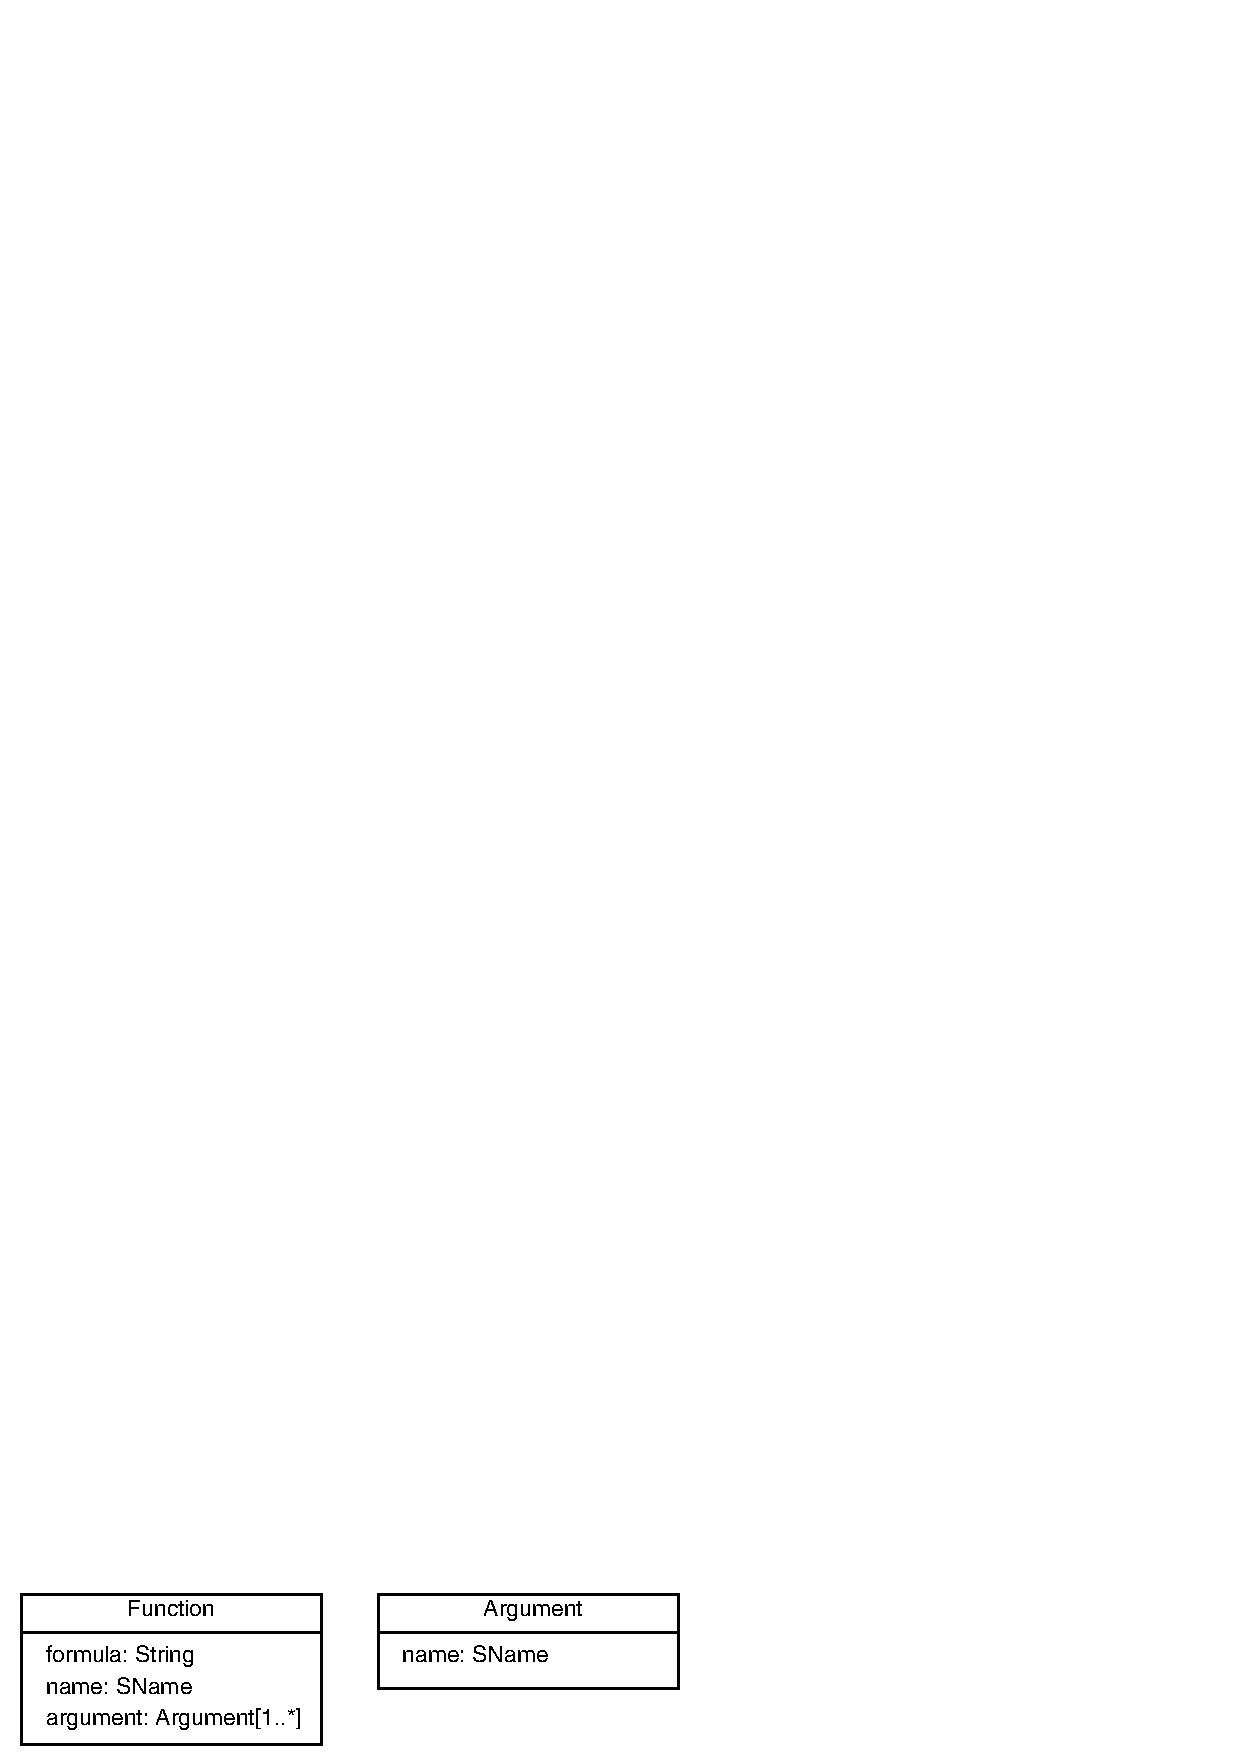
\includegraphics[scale = 0.7]{function}
  \caption{The definition of the \texttt{Function} type.}
  \label{fig:function}
\end{figure}

The \texttt{Function} data structure consists of the function's name
(with a type of \texttt{SName}), a formula string, and a list of
\texttt{Argument} structures.  An \texttt{Argument} structure simply
consists of the argument's name.

The \texttt{Function} structure defines a new function that can be used in
any formula located after the definition of that \texttt{Function}
structure in the text of an SBML model.  The only symbols that can be used
in the \texttt{formula} string of \texttt{Function} are the following:
\begin{itemize}
\item any of the names given in the \texttt{Argument} list;
\item any of the names given in preceding \texttt{Function} structures;
\item any of the names of built-in functions.
\end{itemize}
These restrictions mean that functions cannot be recursive or mutually
recursive, thus ensuring that function ``calls'' can be expanded in place.
Models using functions can therefore be mapped to SBML Level 1.

A \texttt{Function} formula simply returns a \texttt{double} value.  All
the arguments to a function are of type \texttt{double}.  These functions
share the same namespace as other model-level components; this means that,
for example, a function can't have the same name as a specie or a reserved
name.

\subsubsection{Example}

The following is a simple example of a \texttt{Function}
structure in a \texttt{Model} structure:

\begin{example}
<model name="cell">
    <listOfFunctions>
        <function name="pow3" formula="x^3">
            <listOfArguments>
                <argument name="x"/>
            </listOfArguments>
        </function>
    </listOfFunctions>
    ...
</model>
\end{example}

\subsubsection{Issues}
\label{sec:function-issues}

\begin{itemize}

\item Is the scope of symbols in formulas in functions too restrictive?
  
\item Do we need to be able to handle objects other than \texttt{double}
  values?
  
\item Should we actually introduce two kinds of user-defined functions,
  macros and true functions?  The \texttt{Function} proposed above are
  actually macros and can be implemented as text substitutions.  True
  functions would support more than a single \texttt{formula} expression.
  It may be useful to have the ability to define functions as a list of
  expressions, so that functions could compute intermediate values or
  subexpressions within their body.  Without this, it will not be possible
  to split up a complicated expression except by using multiple
  \texttt{Function} definitions.

  Here is an example of what a true function might look like:
\begin{example}
<listOfFunctions>
  <function name="sillyfunction">
    <listOfArguments>
      <argument name="x"/>
      <argument name="y"/>
    </listOfArguments>    
    <listOfParameters>
      <parameter name="a" value="0.5"/>
    </listOfParameters>
    <listOfStatements>
      <statement lhs="a" rhs="cos(x)"/>
      <statement lhs="y" rhs="sin(a)"/>
    </listOfStatements>
  </function>
</listOfFunctions>
\end{example}

\end{itemize}


\subsection{Metadata}
\label{sec:metadata}

The CellML group has worked out an approach to incorporating metadata in
CellML models~\citep{cuellar:2002}.  For SBML Level~2, we propose to use a
subset of the metadata components used in CellML, specifically RDF and the
Dublin Core Metadata Element Set only.  We leave the remaining aspects of
CellML's metadata definition to SBML Level~3.

\subsubsection{Motivations for the Approach}

There are several motivations for taking his approach:
\begin{itemize}

\item RDF plus Dublin Core is not complicated.  If the SBML group were to
  define their own metadata tags, for example, it would undoubtedly end up
  very similar to the Dublin Core set (modulo differences in tag names and
  XML namespaces).
  
\item RDF and Dublin Core are gaining ground as standards.  It is
  preferable to reuse standards when possible rather than proposing unique
  new definitions.  Among other things, this makes it more likely to find
  off-the-shelf tools that work with the standard representations.  There
  currently exist several free RDF parser implementations for Java, C,
  Perl, and other languages.
  
\item A number of other XML-based languages also use RDF for metadata; for
  example, CellML and CML (Chemical Markup Language;
  \url{www.xml-cml.org}).  Settling on the same metadata representation
  would provide greater interoperability as well as opportunities for
  synergies that the SBML community cannot yet anticipate.
 
\item SBML can be specialized to the business of defining biochemical
  models, because SBML is intended to be used by software created for the
  purpose of handling biochemical models.  However, metadata about an SBML
  model is intended to be used not just by these software tools but by
  other software that is \emph{not} specialized to biochemical
  modeling---for example, search engines and database systems.  Thus, it
  behooves us to use a more general framework that is accepted by a broader
  range of software systems.

\item The CellML group has researched the metadata topic extensively.  The
  SBML community can leverage their work and save considerable (and quite
  likely needless) effort.
  
\item Using the same basic metadata framework for both CellML and SBML
  would allow the two dominant biochemical model representation languages
  to be described in common ways, benefitting biologists and other users.

\end{itemize}


\subsubsection{Metadata Components for SBML Level~2}

As mentioned above, we propose using a subset of the CellML metadata
definition, specifically the use of RDF and ``simple'' Dublin Core (i.e.,
the DC Metadata Element Set).  We also propose that the use of these
components in SBML be consistent with their use in the CellML metadata
framework.

Here is an example of XML metadata expressed using this approach (taken
from the CellML metadata specification):
\begin{example}
<rdf:RDF xmlns:dc="http://purl.org/dc/elements/1.1/"
         xmlns:rdf="http://www.w3.org/1999/02/22-rdf-syntax-ns#">
  <rdf:Description rdf:about="#toon_times">
    <dc:title>Toonville Times</dc:title>
    <dc:creator>R.J. Gopher</dc:creator>
    <dc:date>2001-10-18</dc:date>
  </rdf:Description>
</rdf:RDF> 
\end{example}

In the example above, \texttt{dc} is the prefix for Dublin Core elements.
Dublin Core defines the following terms:
\begin{center}
\begin{tabular}{>{\ttfamily}l>{\ttfamily}l>{\ttfamily}l}
Title		& Creator 	& Subject \\
Description 	& Publisher	& Contributor \\
Date		& Type 		& Format \\
Identifier 	& Source	& Language \\
Relation	& Rights	& Coverage\\
\end{tabular}
\end{center}
For information about the specific meanings of these terms, we refer
readers to the CellML Metadata 1.0 Specification
document~\citep{cuellar:2002}.


\subsubsection{Metadata Components for SBML Level~3 and Beyond}

We propose the possible adoption of the remainder of the CellML metadata
elements (e.g., the use of vCard, BQS, etc.) be left to SBML Level~3.  The
goal here is to strike a balance between a larger metadata framework
(namely, the whole of the CellML metadata definition) and none at all.
Hopefully, RDF and Dublin Core can serve as a small-enough working set for
the immediate future.

%\subsubsection{Compatibility with SBML Level~1}

%Because metadata encoded using RDF involves the use of a specific set of
%XML namespaces, and because XML parsing standards dictate that an
%application may ignore XML tags that it does not understand, the proposed
%metadata extension by itself is actually backwards compatible with SBML
%Level~1.


\section{Discussion}

An alternative to the approach taken here is to modularize the definition
of SBML Level~2.  In this alternative approach, each feature (such as
support for arrays, support for spatial geometries, etc.)  would be
encapsulated as a separate add-on, and each SBML Level~2 model would
declare which particular feature set it uses.  A given simulation tool
could key off the feature set declaration in an SBML model file to
determine whether it can interpret the model correctly or whether the model
uses features that it cannot handle.  This is a valid alternative and could
be implemented using a variety of possible mechanisms (e.g., XML
namespaces, or a list of feature tags in an SBML model file header).

Such a modular Level 2 definition may offer advantages in terms of
backwards compatibility.  In particular, note that the additions described
in Sections~\ref{sec:encoding} and~\ref{sec:metadata} (i.e., name encoding
and metadata) are backwards compatible with SBML Level~1.  If a feature-set
approach were used for Level~2, and if a model definition used only these
two Level~2 extensions, the resulting model definition could in fact be
read by an application that only understands SBML Level~1.  This is not
true for the current non-modular Level~2 proposal: without feature-set
tags, an application would either have to assume that it could not handle
the model (because the model says it is a Level~2 definition), or it would
have to parse the whole model definition to evaluate whether it could
handle it.

The present Level~2 proposal does not use this approach primarily for the
following reason: our instinct is that a single cohesive SBML Level~2
definition, rather than a modular one, will be simpler to evaluate by the
community and can be adopted (or rejected) more quickly.

Nevertheless, we propose that this issue (whether to have a singular
Level~2 definition or a modular one) be left to the community to discuss
and evaluate.  This document proposes one a single (non-modular) definition
for Level~2, but the definition could easily be turned into a version
employing feature sets.


%\item A modular definition implies that feature sets are allowed to be used
%  either separately or together, possibly in arbitrary combinations.  This
%  means that more design effort has to be put up-front into good
%  compartmentalization of the feature sets, so that each can stand on its
%  own and be used \emph{sensibly} in combination with others.  For some
%  feature sets, it may prove to be difficult to anticipate the possible
%  interactions between them.


%=============================================================================
% References.
%=============================================================================

\bibliographystyle{apalike}
\bibliography{strings,a,b,c,d,e,f,g,h,i,j,k,l,m,n,o,p,q,r,s,t,u,v,w,x,y,z}

%=============================================================================
% The end.
%=============================================================================

\end{document}
